\section{Descripción del prototipo}
En el siguiente prototipo, de acuerdo al alcance definido en el cronograma realizado al inicio del proyecto se planteo hacer el diseño de el conjunto de interfaces necesarias que nos permitieran presentar los resultados del trabajo final haciendo uso de un sitio web.
\\
Por otro lado se estableció que en este prototipo teniendo configurado el ambiente de Big Data completa ya seria posible  desarrollar los algoritmos de minería de datos que se utilizarían para la operación de este sistema.
\\
De acuerdo a la definición hecha durante fases posteriores del proyecto se seleccionaron 2 algoritmos diferentes: KNN e ID3 para ser desarrollados en este prototipo.
\section{Análisis}
\subsection{Análisis del flujo de datos en las pantallas del sistema}
En este punto del proyecto aun se mantenía la visión de que los algoritmos de minería de datos serían reflejados mediante el uso de las pantallas en un sitio web, por lo que se comparo lo que los algoritmos necesitaban para funcionar y como estas necesidades encontradas podrían ser presentadas e integradas como parte del sitio web. \\
Con este análisis se propuso un mapa de navegación en el sitio que podría solventar esta necesidad. \\
Posteriormente se diseño cada una de las pantallas que se buscaba incluir en el mapa de navegación, sin embargo, al cambiar la forma de presentar los resultados finales se tuvo que dejar este trabajo de lado. \\
A pesar de ello,y como este análisis si fue realizado se puede conocer a detalle en la sección \nameref{sitioweb}.\\
En adelante en esta sección no se hablará mas de este trabajo ya que no forma parte de la solución final, por lo que, en el resto de las secciones de este capitulo solamente se hará énfasis en como se llevo a cabo el desarrollo de los algoritmos de minería de datos. 
\subsection{Análisis de los algoritmos de minería de datos}
Los algoritmos KNN e ID3 fueron seleccionados para ser implementados ya que se trata de algoritmos comúnmente utilizados para el análisis de grandes volúmenes de datos y son algoritmos conocidos en la industria los cuales que no se encuentran en fase experimental y sus resultados ya han sido comprobados en múltiples ocasiones.
\\
Por lo que, se sabe que los algoritmos son efectivos y pueden proporcionar resultados valiosos para las empresas que los consumen.
%Referencia
\\
Por lo que se considera que para proporcionar una muestra de los algoritmos que pueden ser soportados por este paradigma de programación y por esta arquitectura de análisis de datos. Los algoritmos seleccionados son una buena demostración y además son comúnmente utilizados por los usuarios expertos que actualmente hacen uso de Big Data.
\\
Además otra particularidad de esta selección es que se trata de 2 tipos de algoritmos distintos: 
\begin{itemize}
	\item Algoritmo de clasificación
	\item Algoritmo de arboles de decisión.
\end{itemize} 

La teoría del funcionamiento de los algoritmos seleccionados en las secciones \nameref{id3} y \nameref{knnmarco} esto de manera tradicional mostrándose un ejemplo para su ejecución.
\\
En la siguiente sección se muestra la descripción de como es que se hace esta implementación haciendo uso del paradigma Map-Reduce. 

\section{Diseño}
\subsection{Algoritmo KNN con el uso de MapReduce}
Como ya se habia explicado anteriormente Map Reduce es una técnica que descompone un trabajo grande en tareas individuales las cuales pueden ser ejecutadas por separado en diferentes computadoras que componen un cluster, y estas al final pueden unir sus resultados individuales para calcular los resultados finales.\\
se explicará que tiene que realizar la función Map y posteriormente la función Reduce para la resolución de este algoritmo.
\\
\textbf{Función Map}: Toma cada una de las lineas que contiene el archivo de entradas y las procesa de manera individual. centrándose en las columnas que quieren ser utilizadas para su evaluación.\\
Buscando que, los datos contenidos dentro de esas columnas puedan ser procesados por el algoritmo KNN es decir, que tengan un valor ya sea Double o Entero. \\
Se utilizará el ejemplo definido en la sección \nameref{knnmarco} para hacer un poco mas evidente el ejemplo y los cambios que tiene al aplicarlo a este paradigma.\\
Se tomará como dato de referencia el mismo dato utilizado para el caso del Algoritmo sin el uso de Map Reduce es decir:
\begin{lstlisting} 
	Altura (cm), Peso (Kg)
	161 , 61 
\end{lstlisting}
Tomando la primera linea de entrada de la tabla de entradas en el ejemplo se tiene:\\ 
\begin{lstlisting} 
	Altura (cm), Peso (Kg), Talla
	158 , 58 , M
\end{lstlisting} 
Se puede validar que los elementos peso y talla si pueden ser utilizados en este algoritmo ya que los valores que los identifican son de tipo numérico. 
\\
Mientras que, para el valor de Talla al tratarse de un valor que no es ni Double ni Entero, no puede ser procesado directamente por el algoritmo. 
\\
Así que por el momento se tomarán en cuenta los valores unicamente correspondientes a Altura(cm) y Peso (Kg).\\
\\
El siguiente paso, será calcular la distancia que existe entre el elemento referencia y la entrada de la tabla que se esta procesando. \\
Este calculo de distancias se efectúa mediante el calculo de la distancia euclidiana entre los 2 elementos, es decir, la formula mostrada en la figura \ref{fig:distanciaEuclidiana2}\\
	\begin{figure}[H]
		\begin{center}
			\hypertarget{fig:distanciaEuclidiana}{\hspace{1pt}}
			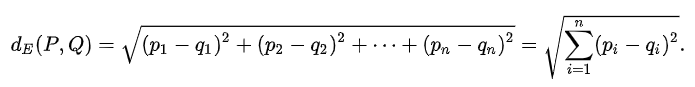
\includegraphics{capitulo2/images/distanciaEuclidiana.png}
			\caption{Fórmula para calcular la distancia Euclidiana.}
			\label{fig:distanciaEuclidiana2}
		\end{center}
	\end{figure} 
Para el caso del ejemplo se tendría el siguiente calculo:
	\begin{figure}[H]
		\begin{center}
			\hypertarget{fig:distanciaejemplo}{\hspace{1pt}}
			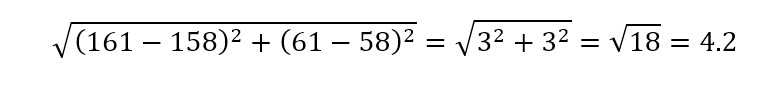
\includegraphics[width=.7\textwidth]{capitulo4a/images/distanciaejemplo.jpeg}
			\caption{Fórmula para calcular la distancia Euclidiana del ejemplo.}
			\label{fig:distanciaejemplo}
		\end{center}
	\end{figure}
Una vez calculada esta distancia, se pasa este calculo a la sección Reduce para que esta continué haciendo los cálculos.
\\
\textbf{Función Reduce}: En esta función se recibe cada una de las lineas que se mandan desde el Map, y se hace un análisis de si este valor ya había sido recibido anteriormente, esto con el objetivo de recibir valores duplicados y manejarlos como un solo elemento. debido a que en este ejemplo no se tienen elementos duplicados esta funcionalidad no sería evidente. \\
Sin embargo la función reduce también ordena todos los resultados obtenidos para todas las lineas entregadas por map. en orden ascendente, es decir, se estaría generando una tabla como la que se muestra a continuación.
	\begin{table}[H]
		\begin{center}
			\label{tab:tablaKNNDistancias}
			\begin{tabular}{c|c|c|c}
				\textbf{Altura (cm)} & \textbf{Peso (kg)} & \textbf{Talla} & \textbf{Distancia}\\
				\hline
				160 & 60 & M & 1.4\\
				163 & 61 & M & 2.0\\
				160 & 59 & M & 2.2\\
				163 & 60 & M & 2.2\\
				160 & 64 & L & 3.2\\
				158 & 59 & M & 3.6\\
				158 & 63 & M & 3.6\\
				163 & 64 & L & 3.6\\
				165 & 61 & L & 4.0\\
				165 & 62 & L & 4.1\\
				158 & 58 & M & 4.2\\
				165 & 65 & L & 5.7\\
				168 & 62 & L & 7.1\\
				168 & 63 & L & 7.3\\
				168 & 66 & L & 8.6\\
				170 & 63 & L & 9.2\\
				170 & 64 & L & 9.5\\
				170 & 68 & L & 11.4\\
			\end{tabular}
		\end{center}
		\caption{Tabla del conjunto de entrenamiento con la columna distancia ya calculada y ordenada.}
	\end{table}  
	Sabiendo el valor del número K, el Reduce toma los primeros K elementos de esta tabla, suponiendo que:
	K=5
	Se generaría la siguiente tabla:
	\begin{table}[H]
		\begin{center}
			\label{tab:tablaKNNDistanciask}
			\begin{tabular}{c|c|c|c}
				\textbf{Altura (cm)} & \textbf{Peso (kg)} & \textbf{Talla} & \textbf{Distancia}\\
				\hline
				160 & 60 & M & 1.4\\
				163 & 61 & M & 2.0\\
				160 & 59 & M & 2.2\\
				163 & 60 & M & 2.2\\
				160 & 64 & L & 3.2\\
			\end{tabular}
		\end{center}
		\caption{Tabla del conjunto de entrenamiento con la columna distancias ya calculada para K=5}
	\end{table}
Posteriormente, se procede a intentar clasificar estos elementos dentro de una clase, suponiendo para este ejemplo en particular que la columna que se quiere considerar para clase es la columna \emph{Talla} entonces, para los 5 k nodos obtenidos se tiene:
\begin{itemize}
	\item 4 Elementos tipo M
	\item 1 Elemento tipo L 
\end{itemize}
Por lo que, finalmente podrían arrojarse los 5 K nodos encontrados y además mencionar que se puede clasificar como un elemento tipo M
\newpage
\subsubsection{Diagrama de Flujo}
Se elaboro un diagrama de flujo que pretende modelar el funcionamiento de este algoritmo como lo hace en el paradigma Map-Reduce. 
el diagrama de flujo generado es el siguiente:
	\begin{figure}[H]
		\begin{center}
			\hypertarget{fig:diagramaflujo}{\hspace{1pt}}
			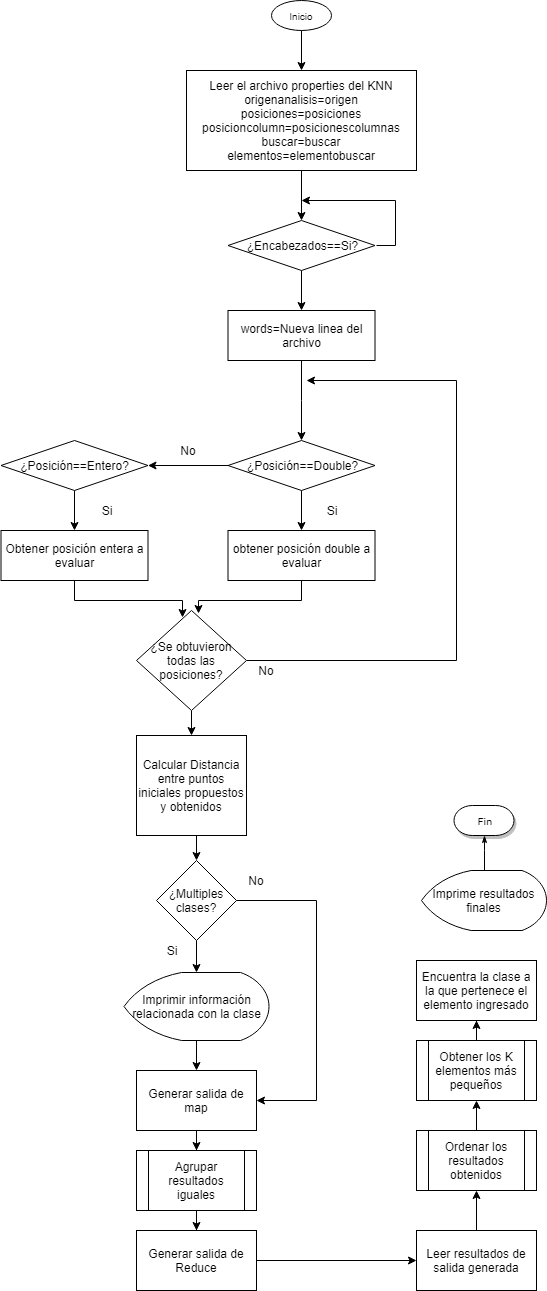
\includegraphics[width=.5\textwidth]{capitulo4a/images/KNN.png}
			\caption{Diagrama de Flujo para el algoritmo KNN.}
			\label{fig:diagramaflujo}
		\end{center}
	\end{figure}
Del diagrama de flujo presentado, se procede a explicar sus pasos:
\\
\begin{enumerate}
	\item Se lee el archivo "Properties" el cual almacena la información de los parámetros de configuración que requiere este algoritmo para empezar a funcionar, es decir. 
	\begin{itemize}
		\item posicionescolumnas:Es el listado de posiciones donde se encuentran el listado de palabras a buscar
		\item Buscar: Este es una bandera la cual sirve para agregar un elemento en particular que se quiera buscar, es decir, de toda la columna que 
		\item Origen: Contiene los datos de referencia sobre los que se quiere buscar, estos tienen que ser del mismo tipo de dato que las columnas de interés del usuario ademas de que deben de encontrarse en el mismo orden en que aparecen en el archivo.
		\item posiciones: Es el listado de los números de columnas que contienen la información que se desea tomar en cuenta para el análisis KNN de la totalidad del archivo.
	\end{itemize} 
\end{enumerate}
%\subsection{Algoritmo ID3}
\newpage
